\chapter{Experiments}
We did several experiments to answer the following questions:
\begin{enumerate}
    \item How stable is the cycle count per iteration?
    \item Is there any overhead for more \acp{pe}?
    \item When using a fixed grid size, how does the performance of using more \acp{pe} compare to using larger tiles on fewer \acp{pe}?
    \item What is the maximum tiling size that fits into the memory of a \ac{pe}?
    \item How does the performance of the generalized algorithm compare to the specialized algorithm for radius 1?
    \item How does the Cerebras implementation compare to highly optimized implementations on traditional \ac{hpc}-Arcitectures (\ac{cpu}, \ac{gpu})?
    \item (How does a 2d stencil compare to a 3d stencil?)
    \item What contributes to the cycle count?
\end{enumerate}

All experiments are performed on the cycle accurate simulator that is part of the Cerebras \ac{sdk}.
Using the simulator limits the number of \acp{pe} and number of iterations so that the data needs to be extrapolated to the whole grid.
We examine to what extend extrapolation is possible in the first two experiments.

We count the cycles used per iteration in the simulator and use this together with the clock speed of the \ac{wse} to calculate the time per iteration.

One difference between the simulator and the real hardware is that the simulator does use a single clock for all cores, while the real hardware has a separate clock for each core. (verify this!!!) Because these clocks are not perfectly synchronized, especially experiments with a large number of \acp{pe} could differ in the cycle count. Although this is not guaranteed for our algorithm, (source) find that in practice the slighly desynchronized clocks improve overall performance compared to the simulator. 

\section{Stability of cycle count per iteration}
For this experiment, we fix the grid size, tile size and radius and run the simulation for different number of iterations.
After two iterations of varying cycle count, the cycle is mostly stable.
For a grid size of 10x10, the cycle count per iteration is $16\pm1$ on \ac{wse}-2 and $23\pm1$ on \ac{wse}-3.

For a grid of 10x10, and a tile size of 1x1 and radius 1, the tiled algorithm achives $127\pm0$ cycles per iteration on \ac{wse}-2 and $156\pm1$ cycles per iteration on \ac{wse}-3.

A larger problem size with a grid of 100x100, tile size of 10x10 and radius 5, results in a cycle count per iteration of $3353\pm20$ on \ac{wse}-2 and $3377\pm5$ on \ac{wse}-3.

Because of the high flucuations in the cycle count in the first two iterations, we measure the cycle count in the following experiments as an average of the 3rd and 4th iteration.

\begin{figure}[h]
    \centering
    \begin{subfigure}[b]{0.48\textwidth}
        \centering
        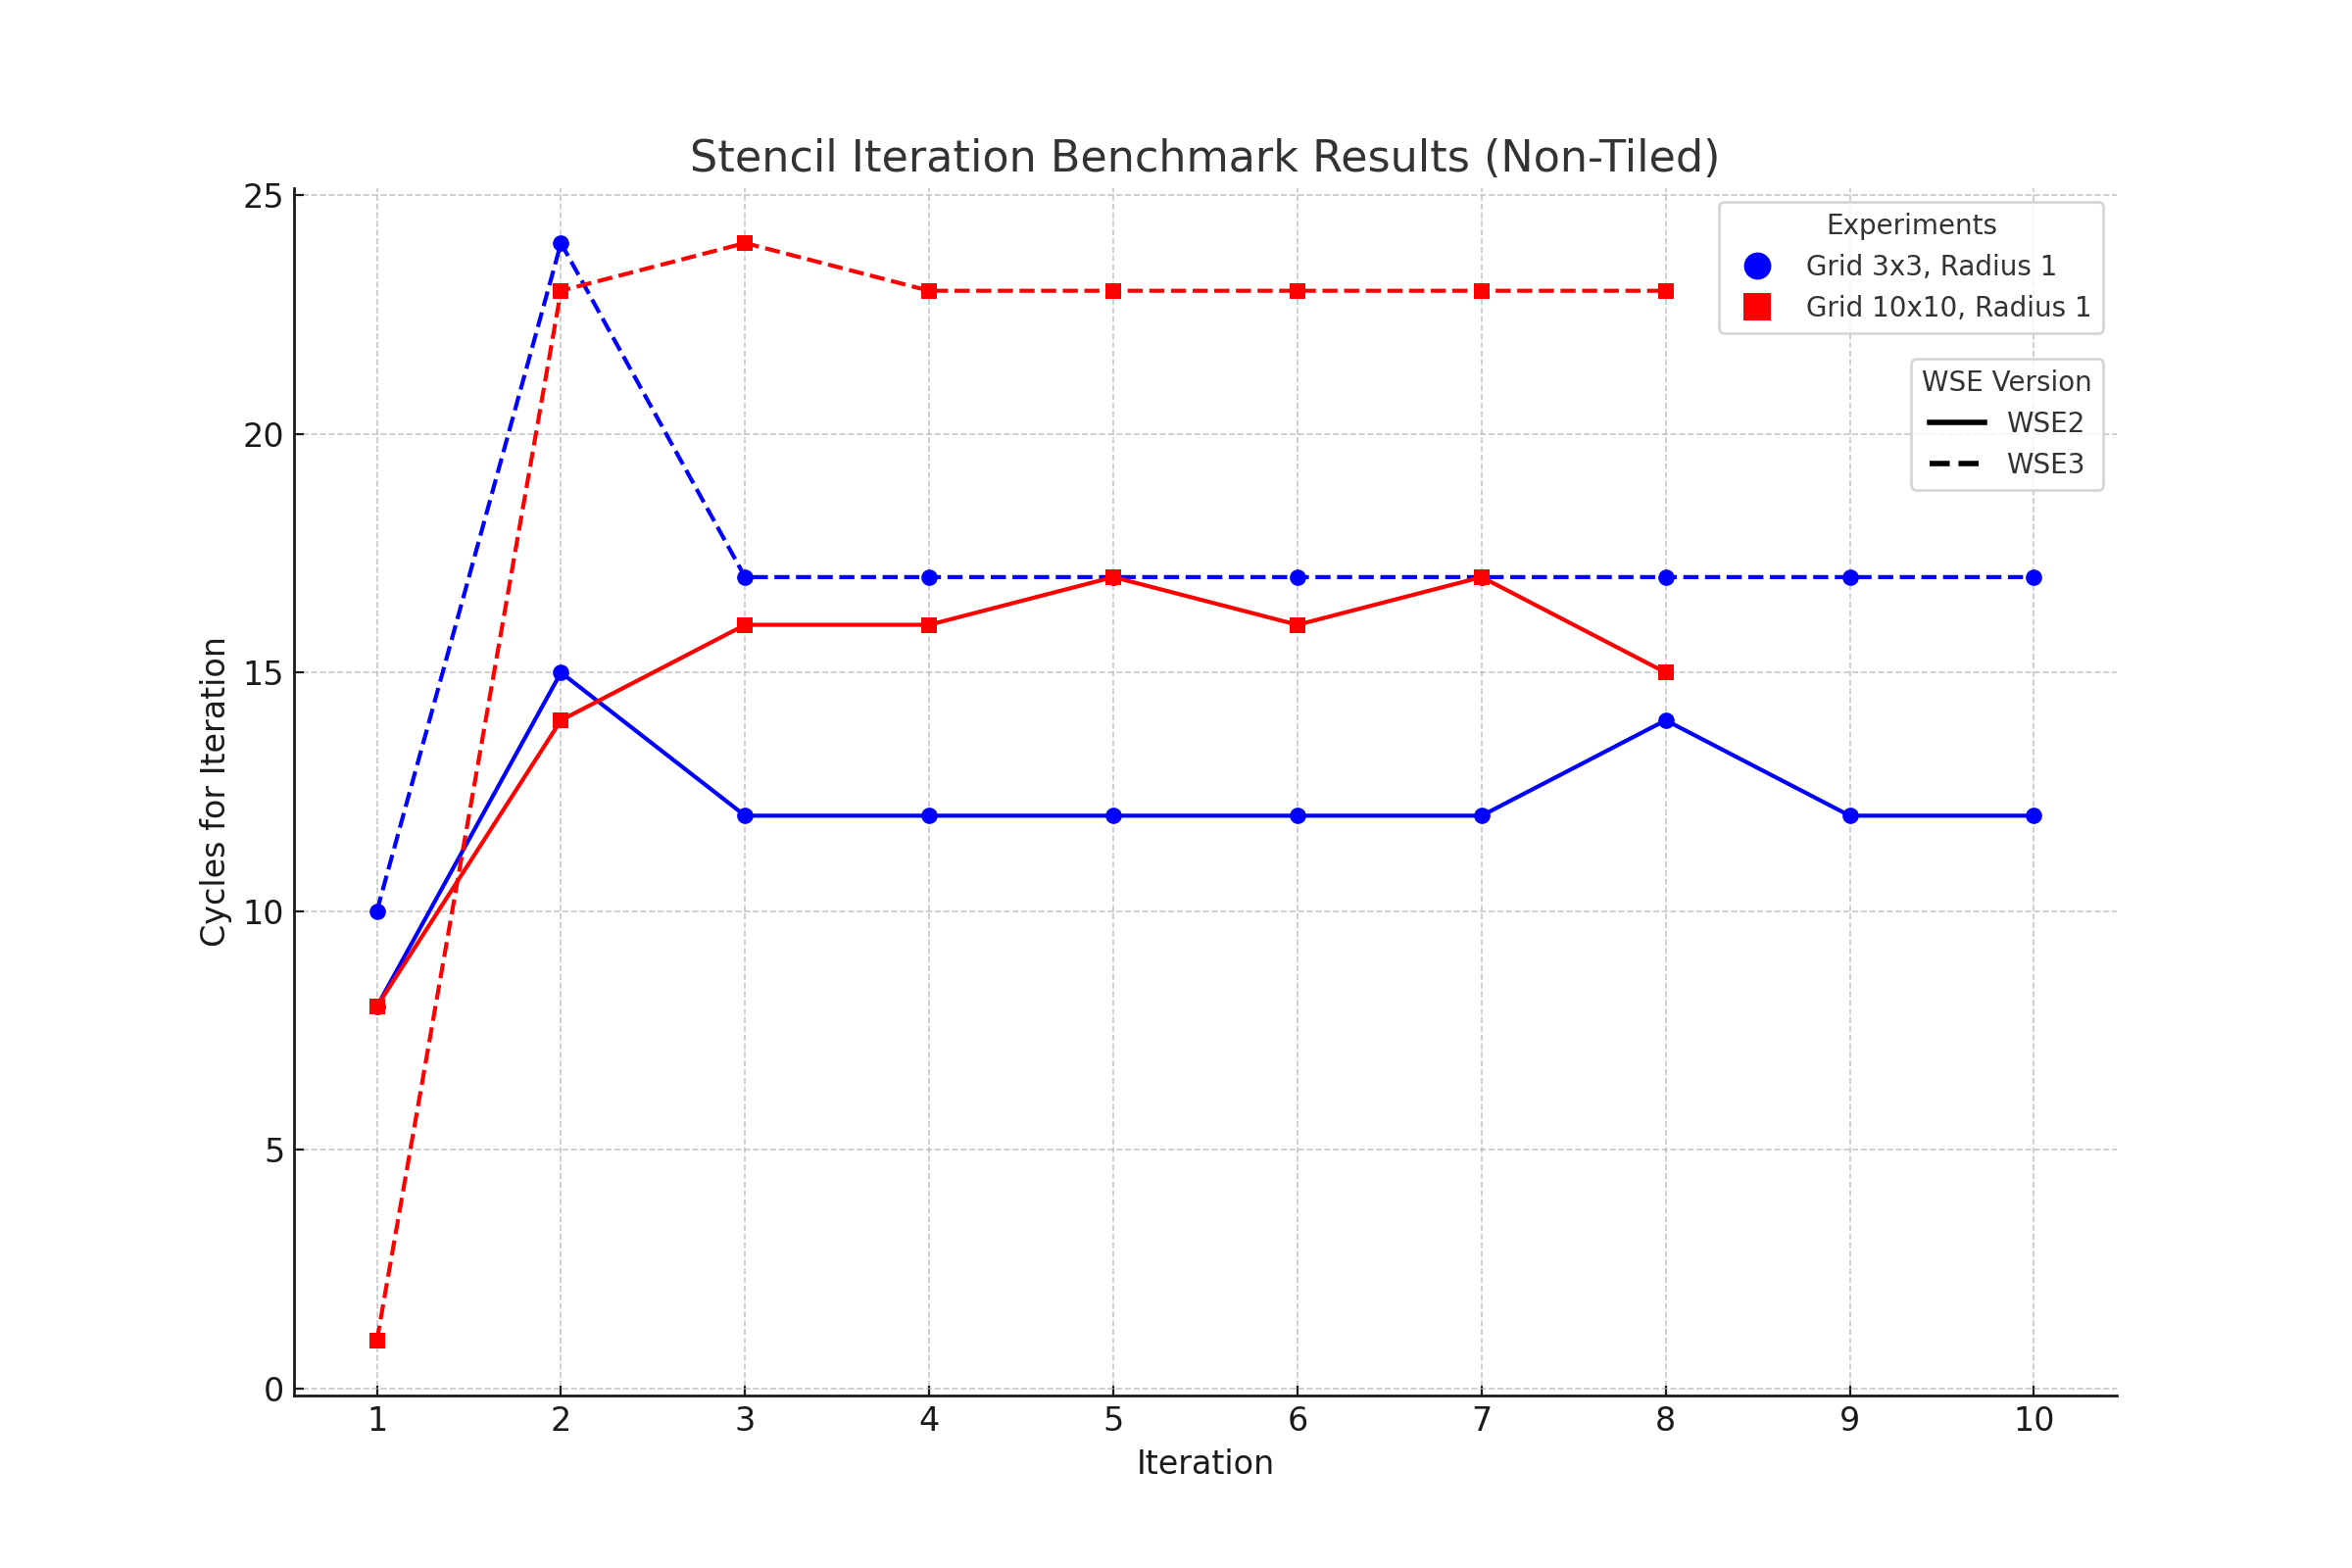
\includegraphics[width=\textwidth]{non_tiled_iteration_stability.png}
        \caption{Non-tiled algorithm}
        \label{fig:non_tiled_iteration_stability}
    \end{subfigure}
    \hfill
    \begin{subfigure}[b]{0.48\textwidth}
        \centering
        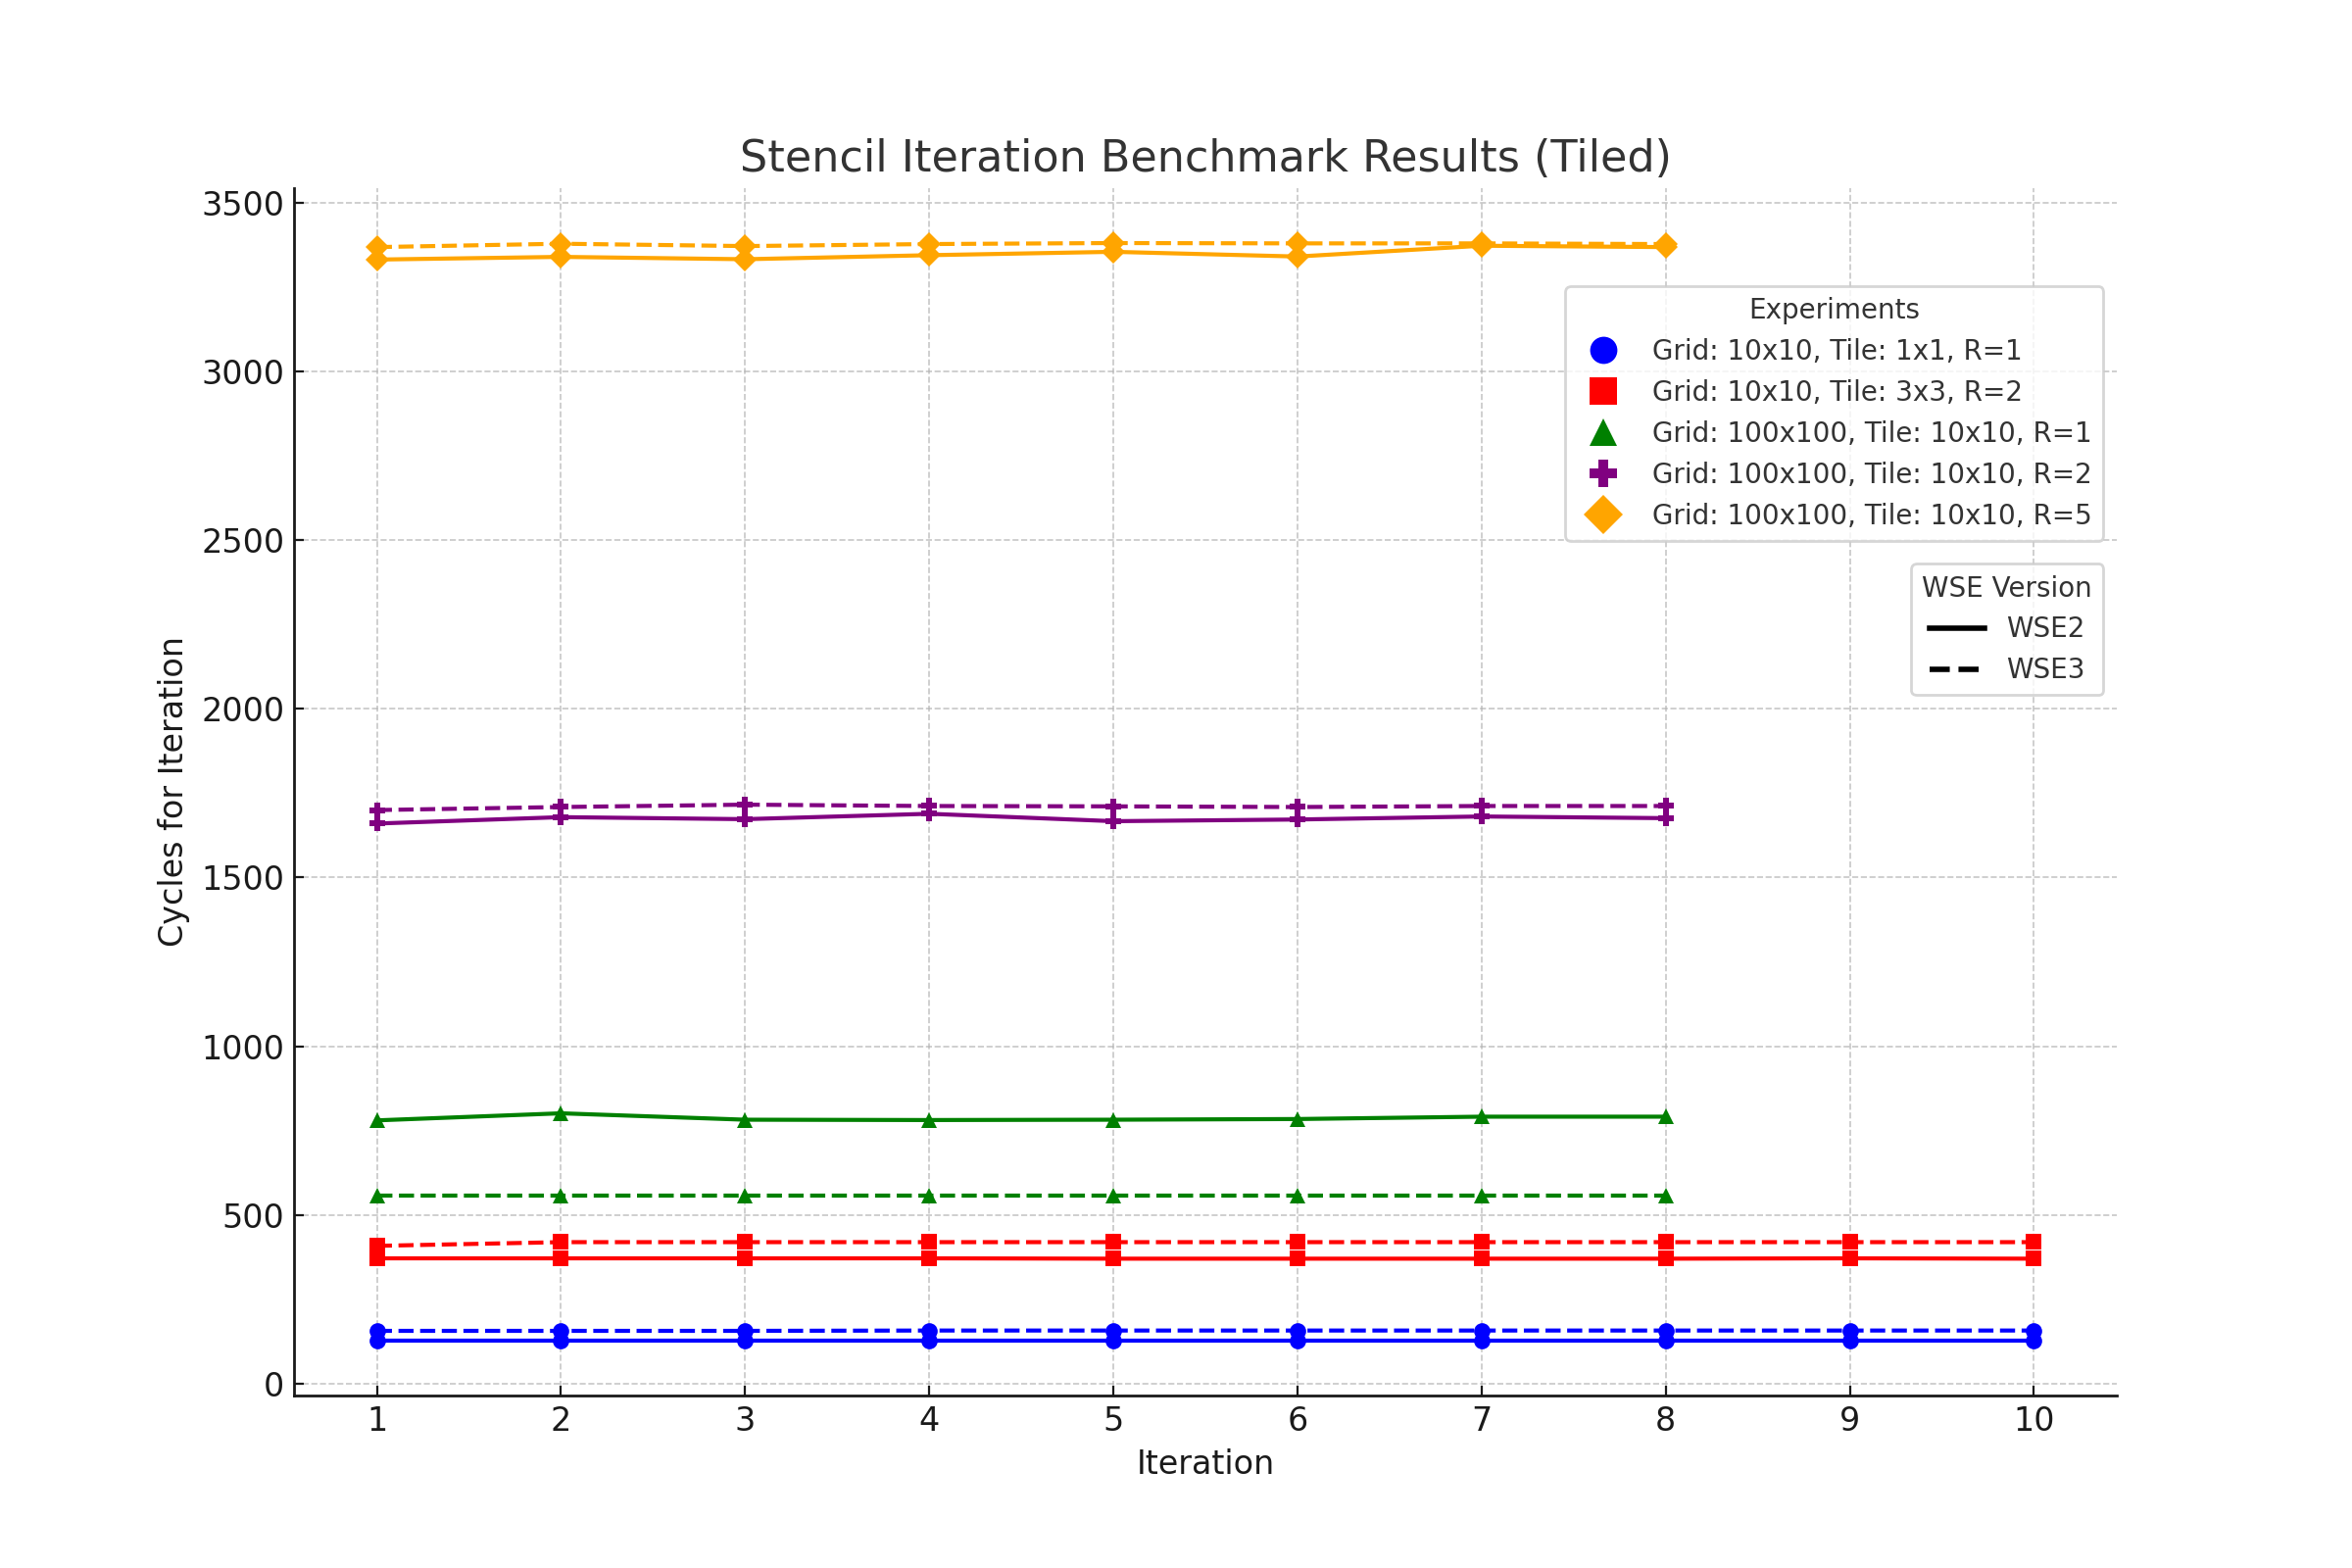
\includegraphics[width=\textwidth]{tiled_iteration_stability.png}
        \caption{Tiled algorithm}
        \label{fig:tiled_iteration_stability}
    \end{subfigure}
    \caption{Cycle count per iteration for non-tiled and tiled algorithm}
    \label{fig:iteration_stability}
\end{figure}



\section{Overhead for more \acp{pe}}
\label{sec:pe_overhead}
A very interesting question is how the performance scales with the number of \acp{pe}.
As each \ac{pe} is independent from the others, the time per iteration should be independent from the number of \acp{pe}.
This can be confirmed by the tests on the simulator up to a \ac{pe} count of \num{2500} (\numproduct{50 x 50}) for the non-tiled algorithm and \num{625} (\numproduct{25 x 25}) for the tiled algorithm.

\begin{figure}[h]
    \centering
    \begin{subfigure}[b]{0.48\textwidth}
        \centering
        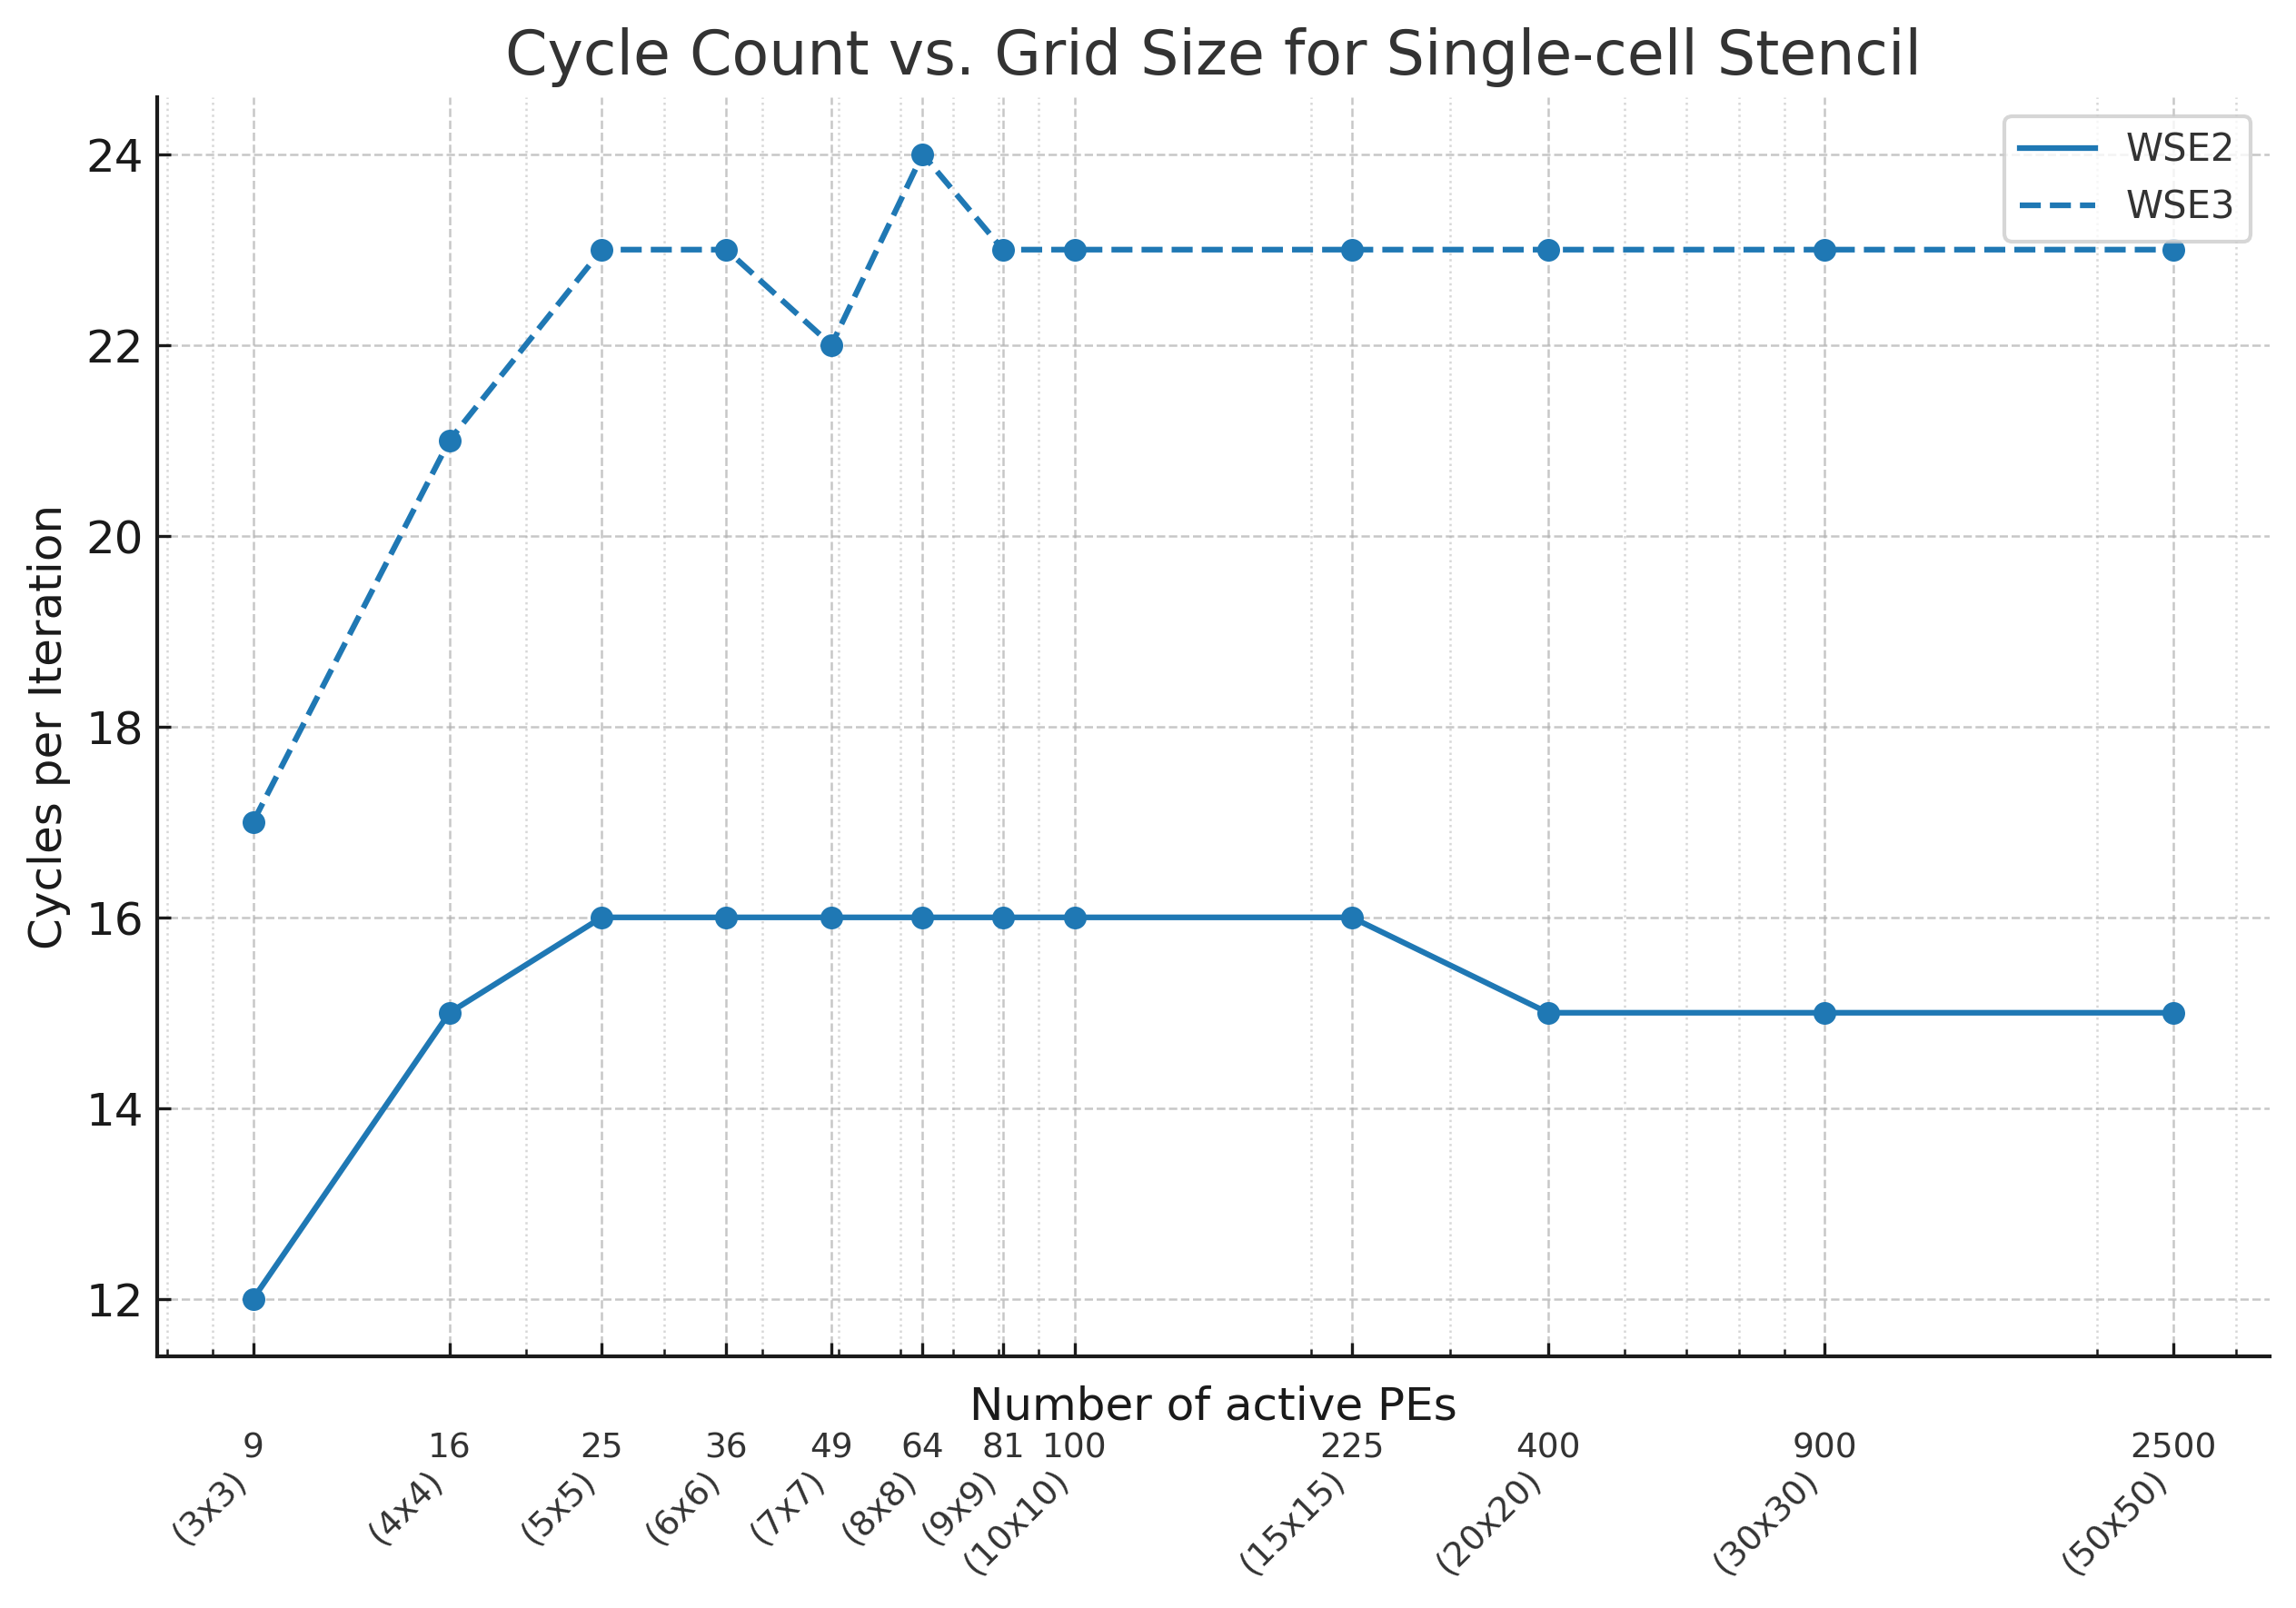
\includegraphics[width=\textwidth]{pe_overhead_non_tiled.png}
        \caption{Non-tiled algorithm}
        \label{fig:pe_overhead_non_tiled}
    \end{subfigure}
    \hfill
    \begin{subfigure}[b]{0.48\textwidth}
        \centering
        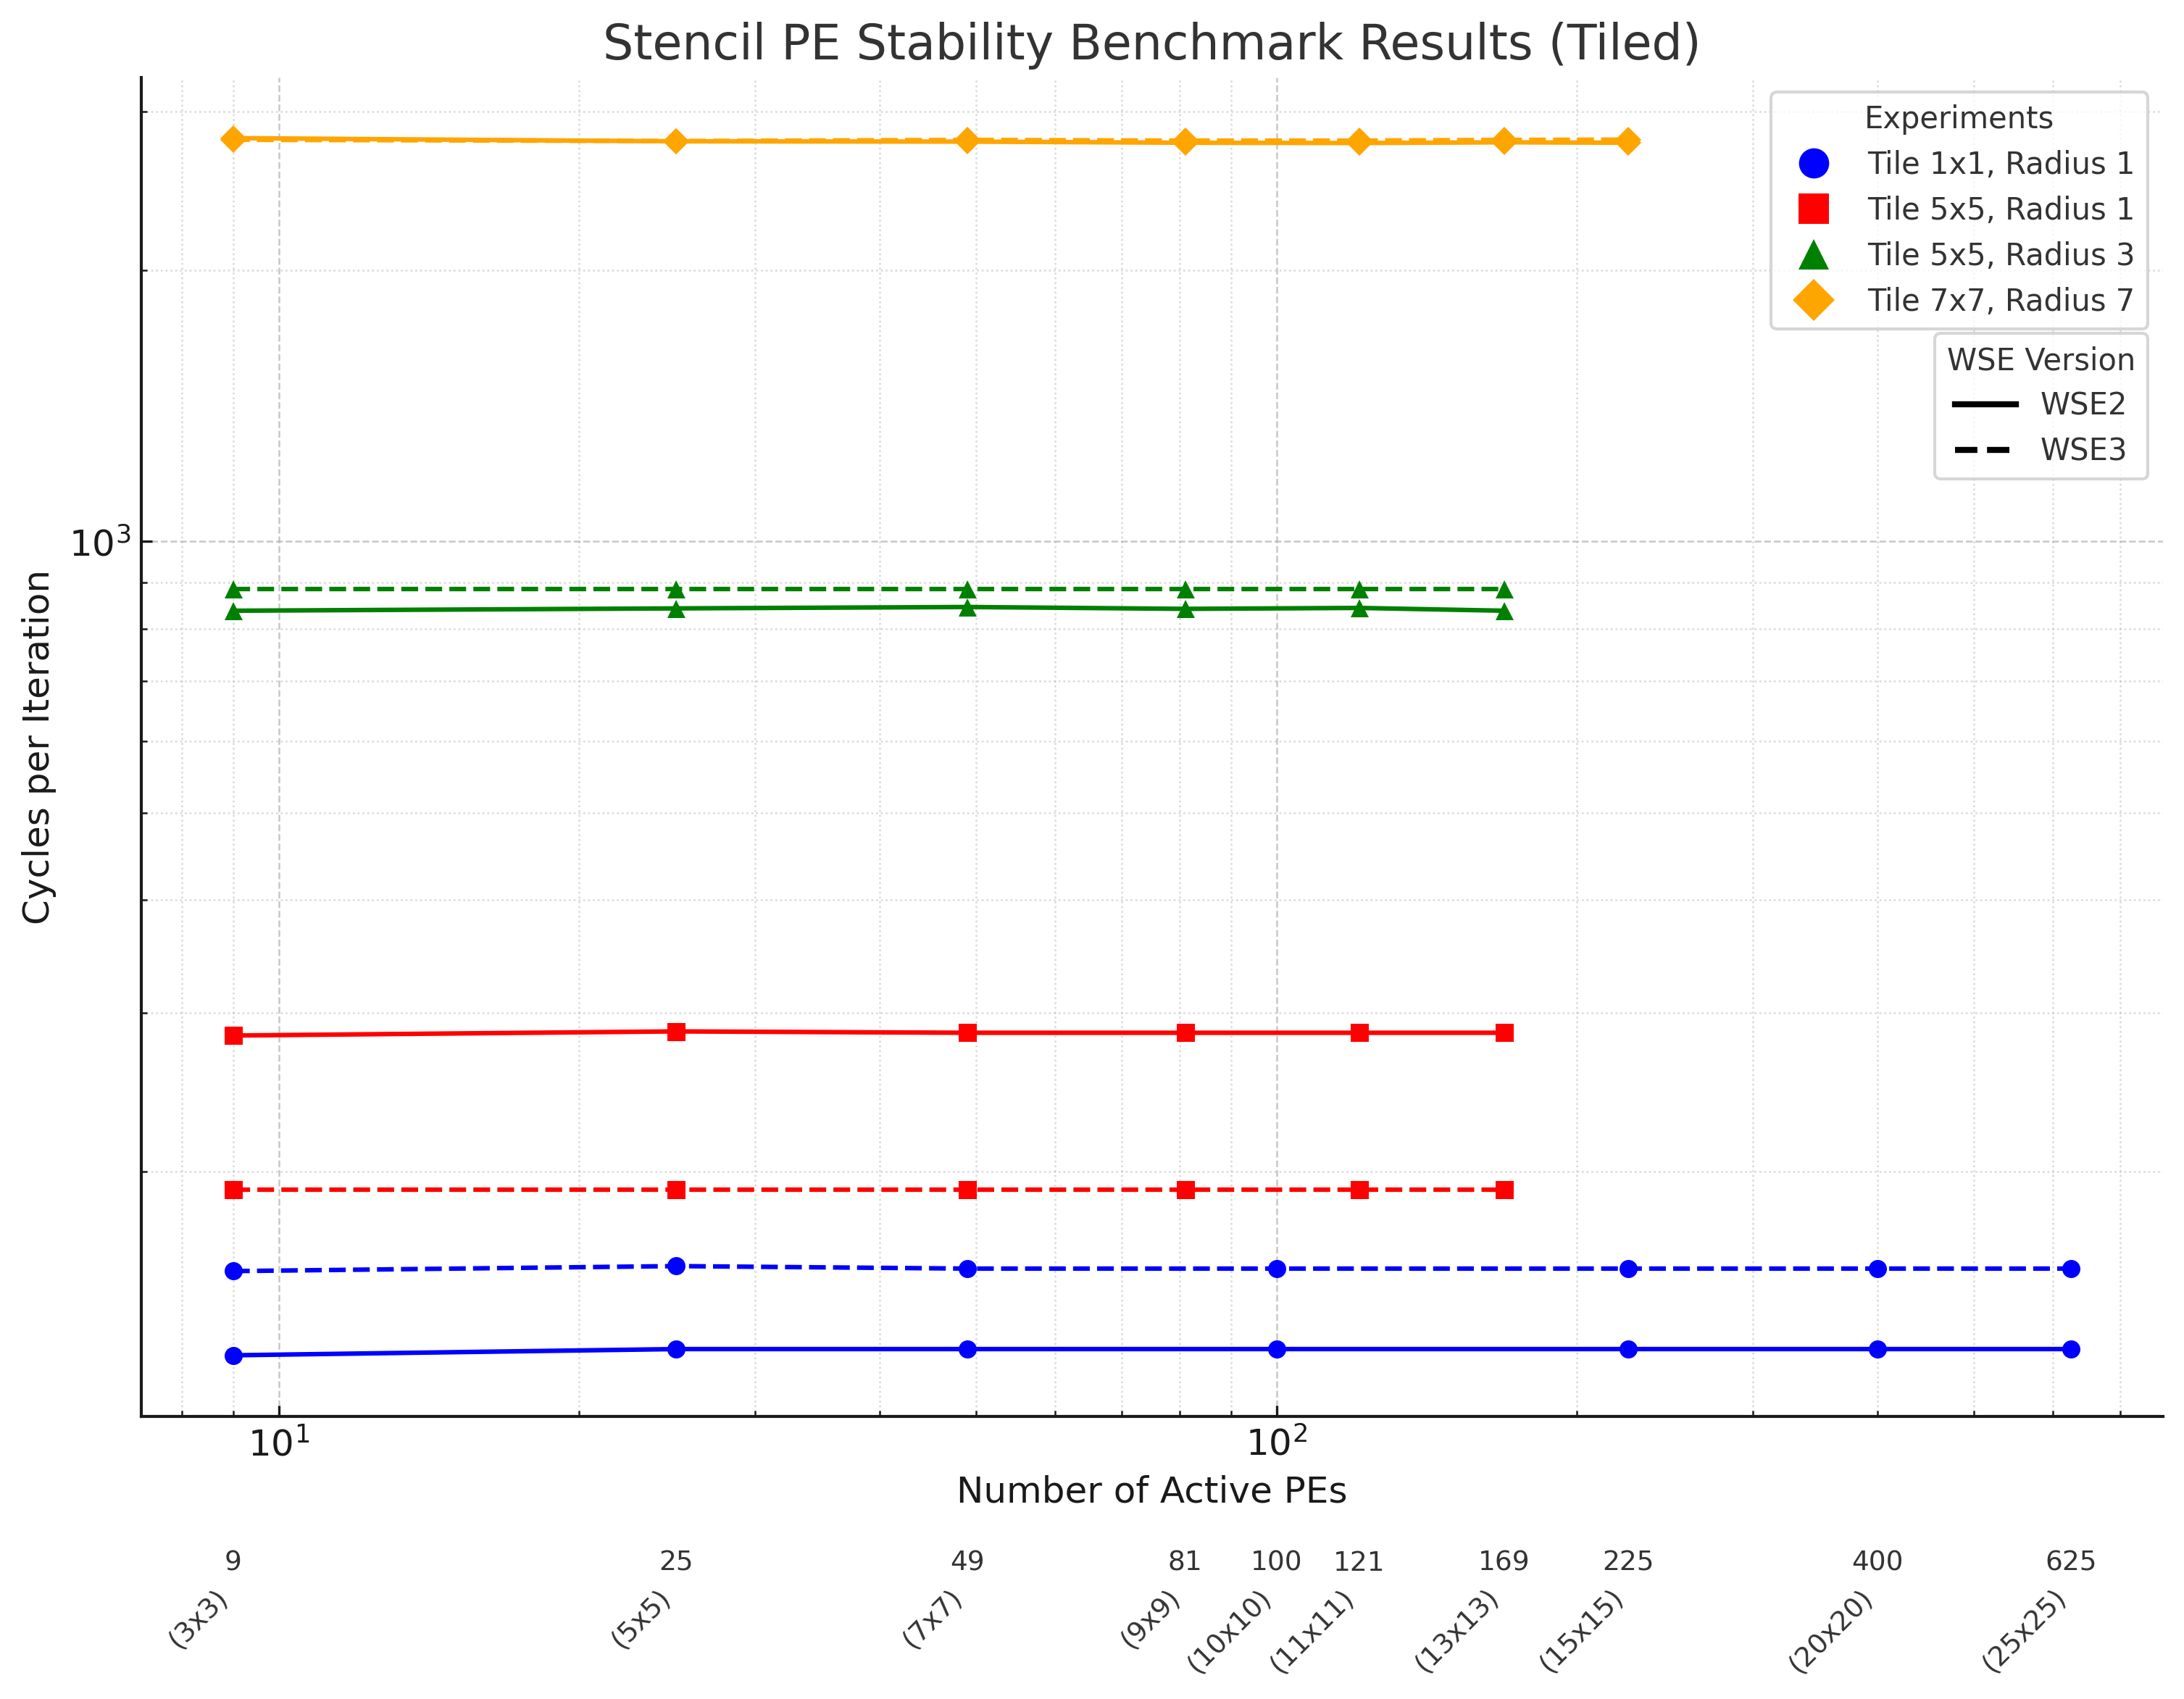
\includegraphics[width=\textwidth]{tiled_pe_stability.png}
        \caption{Tiled algorithm}
        \label{fig:tiled_pe_stability}
    \end{subfigure}
    \caption{Cycle count per iteration versus the number of active PEs for (a) the non-tiled algorithm and (b) the tiled algorithm. For the non-tiled implementation, the performance is stable for grids larger than 4x4, with the 3x3 grid showing a notably lower cycle count. The tiled implementation also demonstrates a consistent cycle count for a given configuration, independent of the number of active PEs.}
    \label{fig:pe_overhead}
\end{figure}

As shown in \autoref{fig:pe_overhead_non_tiled}, the performance of the non-tiled algorithm scales almost perfectly, with the cycle count remaining constant with minimal fluctuations regardless of the grid size. The one exception is the 3x3 grid, which is significantly faster. We hypothesize this is an artifact of the experimental setup where only the single, inner \ac{pe} is performing computation and does not need to synchronize with other computing neighbors, effectively eliminating the communication latency discussed in \autoref{sec:theoretical_performance_evaluation_and_comparison_against_roofline_model}. For all subsequent experiments, we ensure at least \numproduct{5 x 5} active \acp{pe} - which results in at least \numproduct{3 x 3} \acp{pe} inner \acp{pe} - to provide representative results.

\cite{source} shows that for a 3d stencil that is tested on real hardware, the cycle count scales perfectly with the number of \acp{pe} up to the whole \ac{wse} dimensions (verify this!!!).

We therefore expect that our implementation also scales perfectly (or nearly perfectly) on the real hardware.



\section{Maximum tiling size}
The maximum tiling size that fits into the memory of a \ac{pe} is limited by the number of memory banks and the size of the data structure registers.
We test this by increasing the tile size to the maximum that still compiles for (test wse2 and wse3 independently!!! currently same number for both (smaller one))

We find that the maximum tiling size  is 64x64=4096 elements.
A non-quadratical tile size, that results in 4096 elements, is likely also possible, but not tested.
Tile size of 64x64 was tested up to radius 3. It is likely to decrease for larger radius.

This results in a maximum grid size of 48000x51000 on wse-2 and 48000x76000 on wse-3. (calculate correct number here!!!)

\section{Comparison of non-tiled and tiled algorithm}

The non-tiled algorithm is implemented in a completely different way than the tiled algorithm.
This allows for a very optimized implementation, that doesn't require any runtime \ac{dsd} to \ac{dsr} transfers, asynchronous operations and task activation.
It is therefore significantly faster than the tiled algorithm for radius 1.
However, the non-tiled algorithm is naturally limited to a radius of 1 and a grid size not larger than the \ac{wse} dimensions.

\begin{figure}[h]
    \centering
    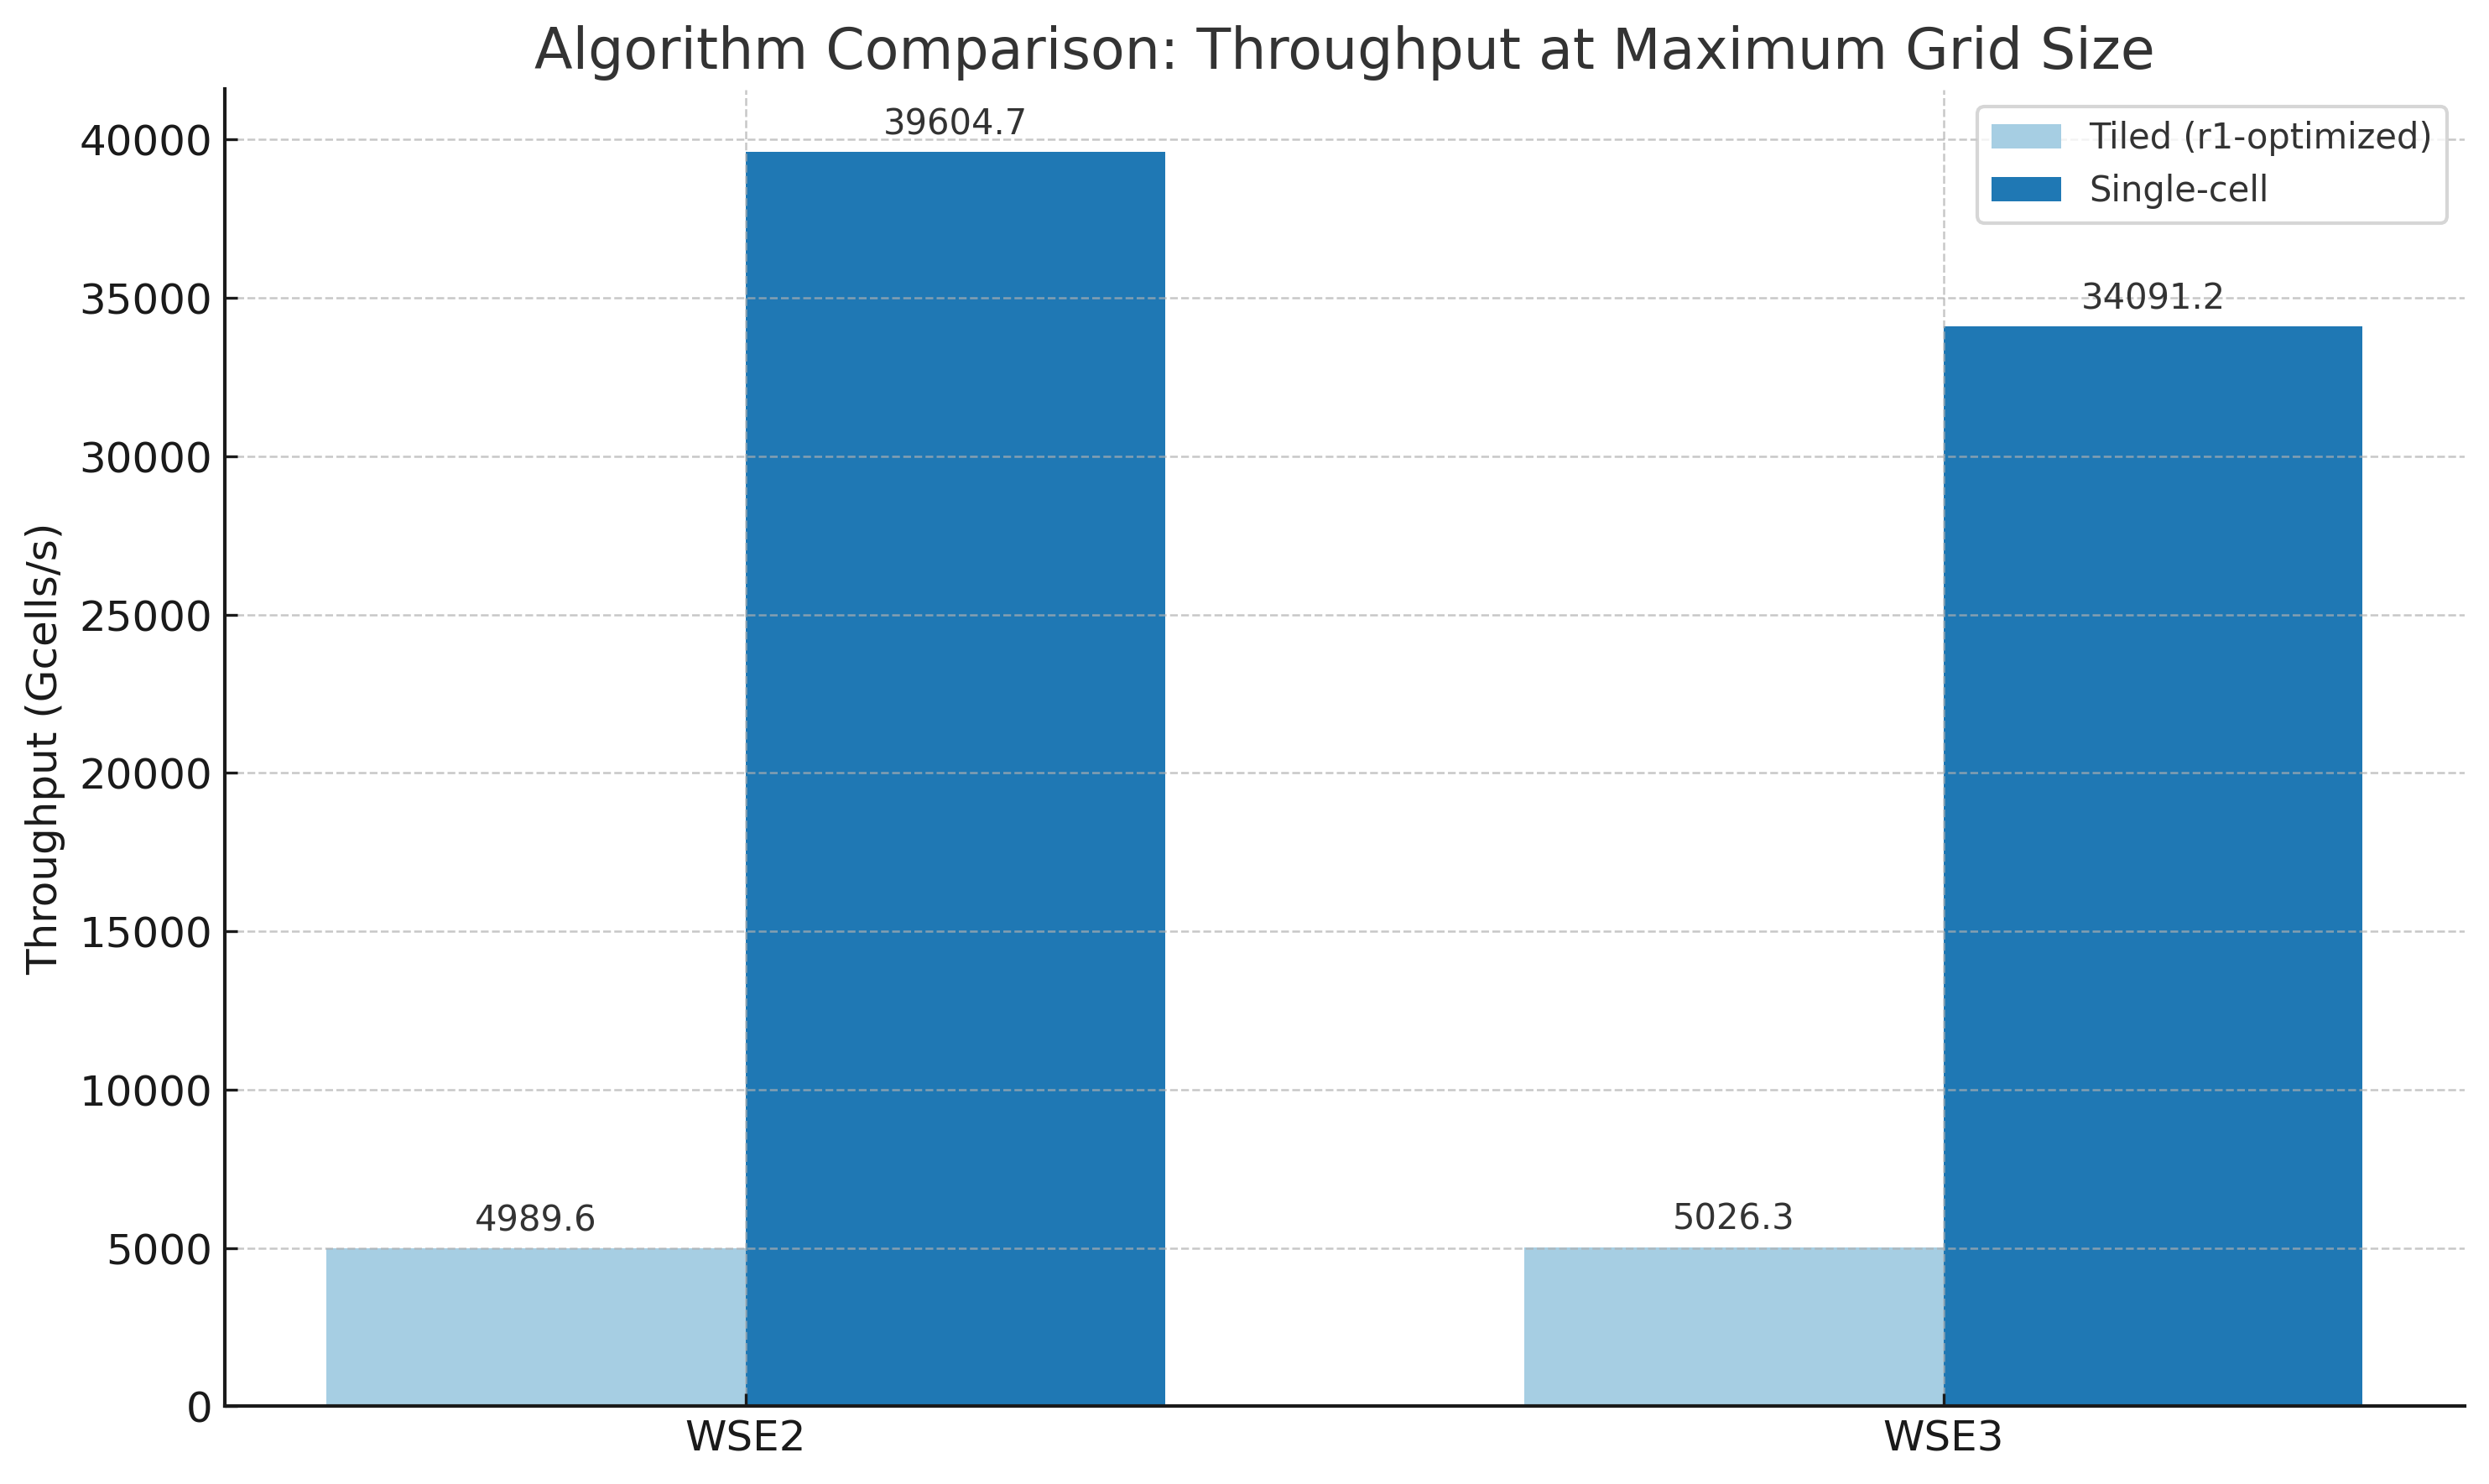
\includegraphics[width=0.5\linewidth]{algo_comparison.png}
    \caption{Performance comparison of the specialized non-tiled and the r1-optimized tiled implementations for a radius-1 stencil. The specialized, non-tiled algorithm is significantly faster, achieving an 8x speedup on \ac{wse}-2 and a 7x speedup on \ac{wse}-3 due to its simpler communication and execution model.}
    \label{fig:algo_comparison}
\end{figure}

\section{Comparison of Cerebras and traditional \ac{hpc}-Arcitectures}
We conducted several experiments to compare the performance of the implemented stencils on the Cerebras \ac{wse} with highly optimized Devito implementations on \ac{cpu} and \ac{gpu}. The experiments were conducted in Vast.ai cloud.
As a \ac{cpu} we used AMD EPYC 9554 64-Core Processor.
As a \ac{gpu} we used NVIDIA H100 SXM 80GB.

For the first experiment, we ran the optimized stencil code on \ac{cpu} and \ac{gpu} and kept the product of grid size and number of iterations constant. This results in a constant number of total flops. 

\begin{figure}[h]
    \centering
    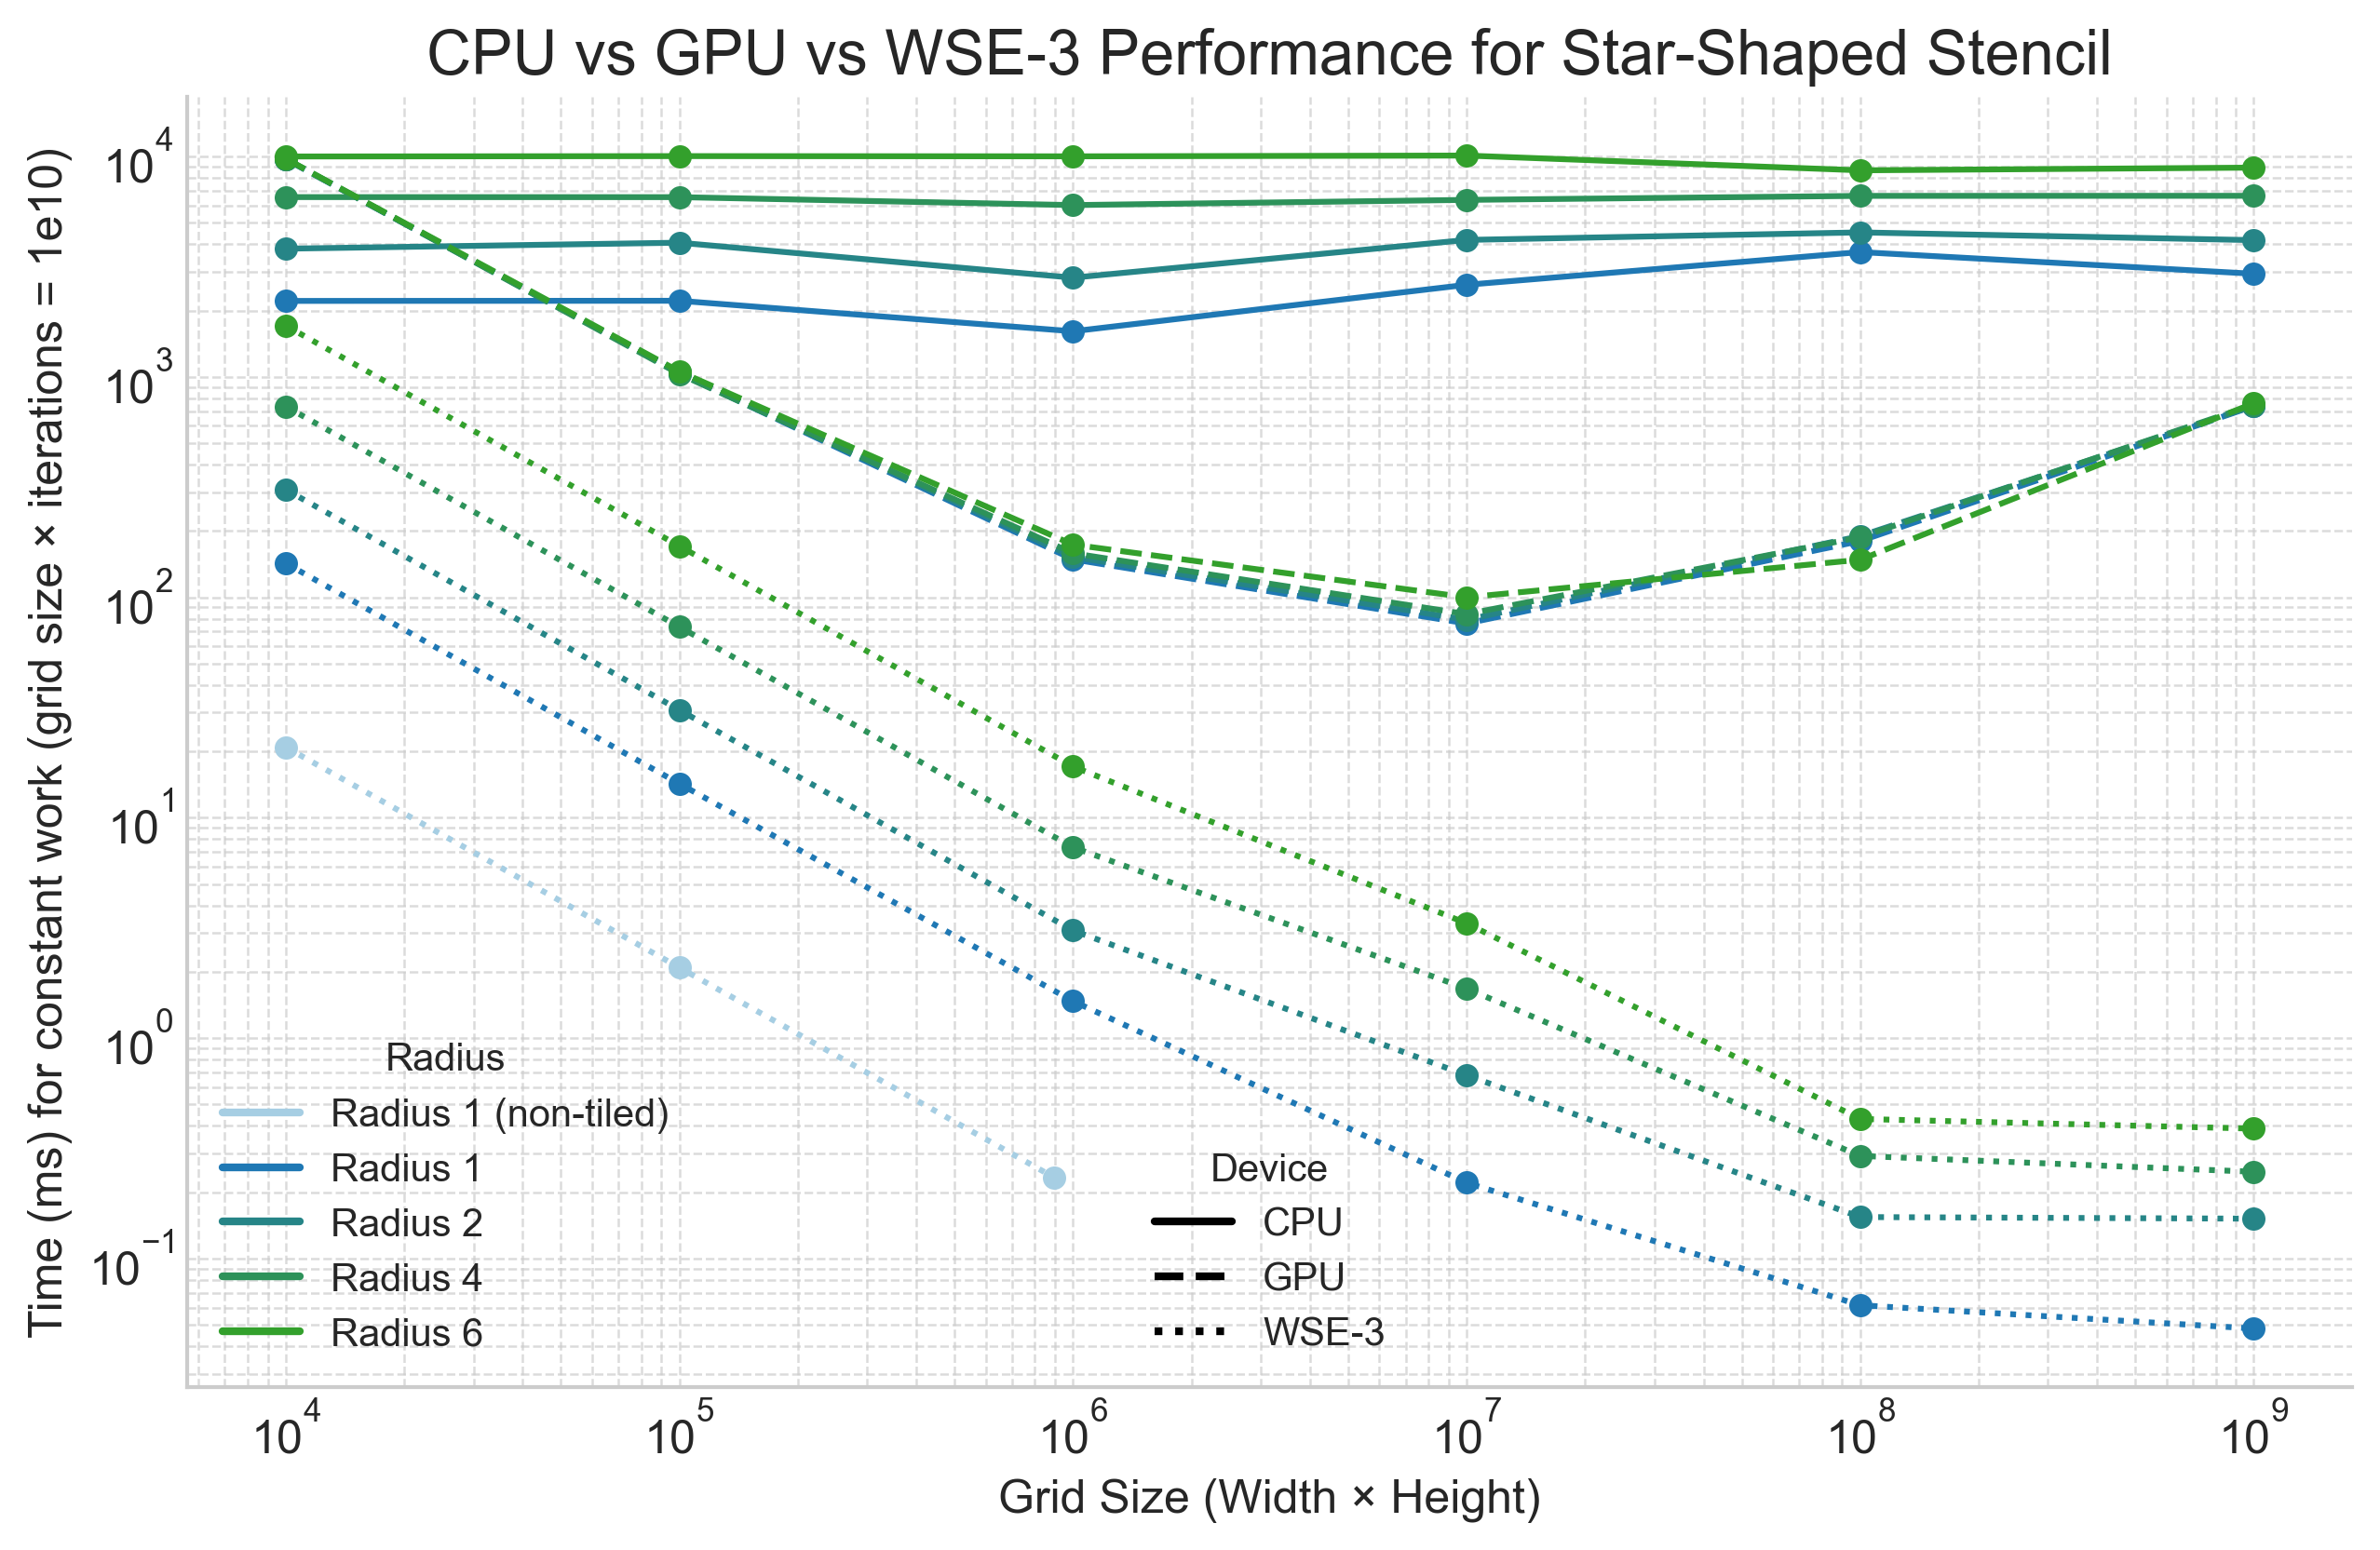
\includegraphics[width=1\linewidth]{gpu_cpu_wse3_constant_product.png}
    \caption{Comparison of \ac{cpu} and \ac{gpu} performance for different grid sizes and number of iterations, so that $width \times height \times iterations = \num{1e10}$}
    \label{fig:gpu_cpu_constant_product}
\end{figure}

The results show that for most tested configurations, the \ac{gpu} outperforms the \ac{cpu}.
However for very small tile sizes of 100x100 and large iteration counts of $\num{1e6}$, the \ac{cpu} is faster.

Furthermore we observe that \ac{gpu} performance differs significantly depending on the racio between grid size and iterations with an optimal performance at $\num{1e3}$ iterations and a grid size of $\num{1e7}$. At this grid size, the data ($\num{1e7}$ numbers $\times$ \qty{4}{\byte} per number $=$ \qty{40}{\mega\byte}) fits perfectly into \qty{50}{\mega\byte} L2 cache of the H100. 

Notably the \ac{gpu} perfors up to 100x worse for non-ideal grid sizes with $\num{1e4}$ elements compared to the ideal grid size with $\num{1e7}$ elements.

For \ac{cpu}, the performance is not as sensitive to the ratio between grid size and iterations with just 2x worse performance for the least ideal grid size of $\num{1e8}$ elements compared to the ideal grid size of $\num{1e6}$ elements.

Another notable observation is that the \ac{cpu} is a lot more sensitive to different radii (which do change the number of flops) than the \ac{gpu}. For the \ac{cpu} and its optimal grid size of $\num{1e6}$, it takes 3.8 times longer to calculate the 4 times as computationally expensive stencil with radius 4 compared to the stencil with radius 1. For the \ac{gpu} on the other hand, it takes only 1.1 times as long for its optimal grid size of $\num{1e7}$.
This indicates that in their optimal configuration, the \ac{cpu} is compute limited while the \ac{gpu} is memory limited.

As a second experiment, we compared our implementation for a grid size of the \ac{gpu}-optimal $\num{1e7}$ to the optimized \ac{gpu} and \ac{cpu} implementation. To fit a size of $\num{1e3}\times\num{1e4}$ on the \ac{wse}-2 with dimensions of $750\times994$, we need a tile size of at least $2x11$ and on \ac{wse}-3 with dimensions of $750\times1200$ a tile size of at least $14x1$. As shown in the earlier experiments, degrade larger tile sizes always the performance so we used these minimum tile sizes. Because of the radius constraint from \autoref{eq:radius_constraint}, we need to increase the shorter dimension of the tile to the respective radius.

\begin{figure}[h]
    \centering
    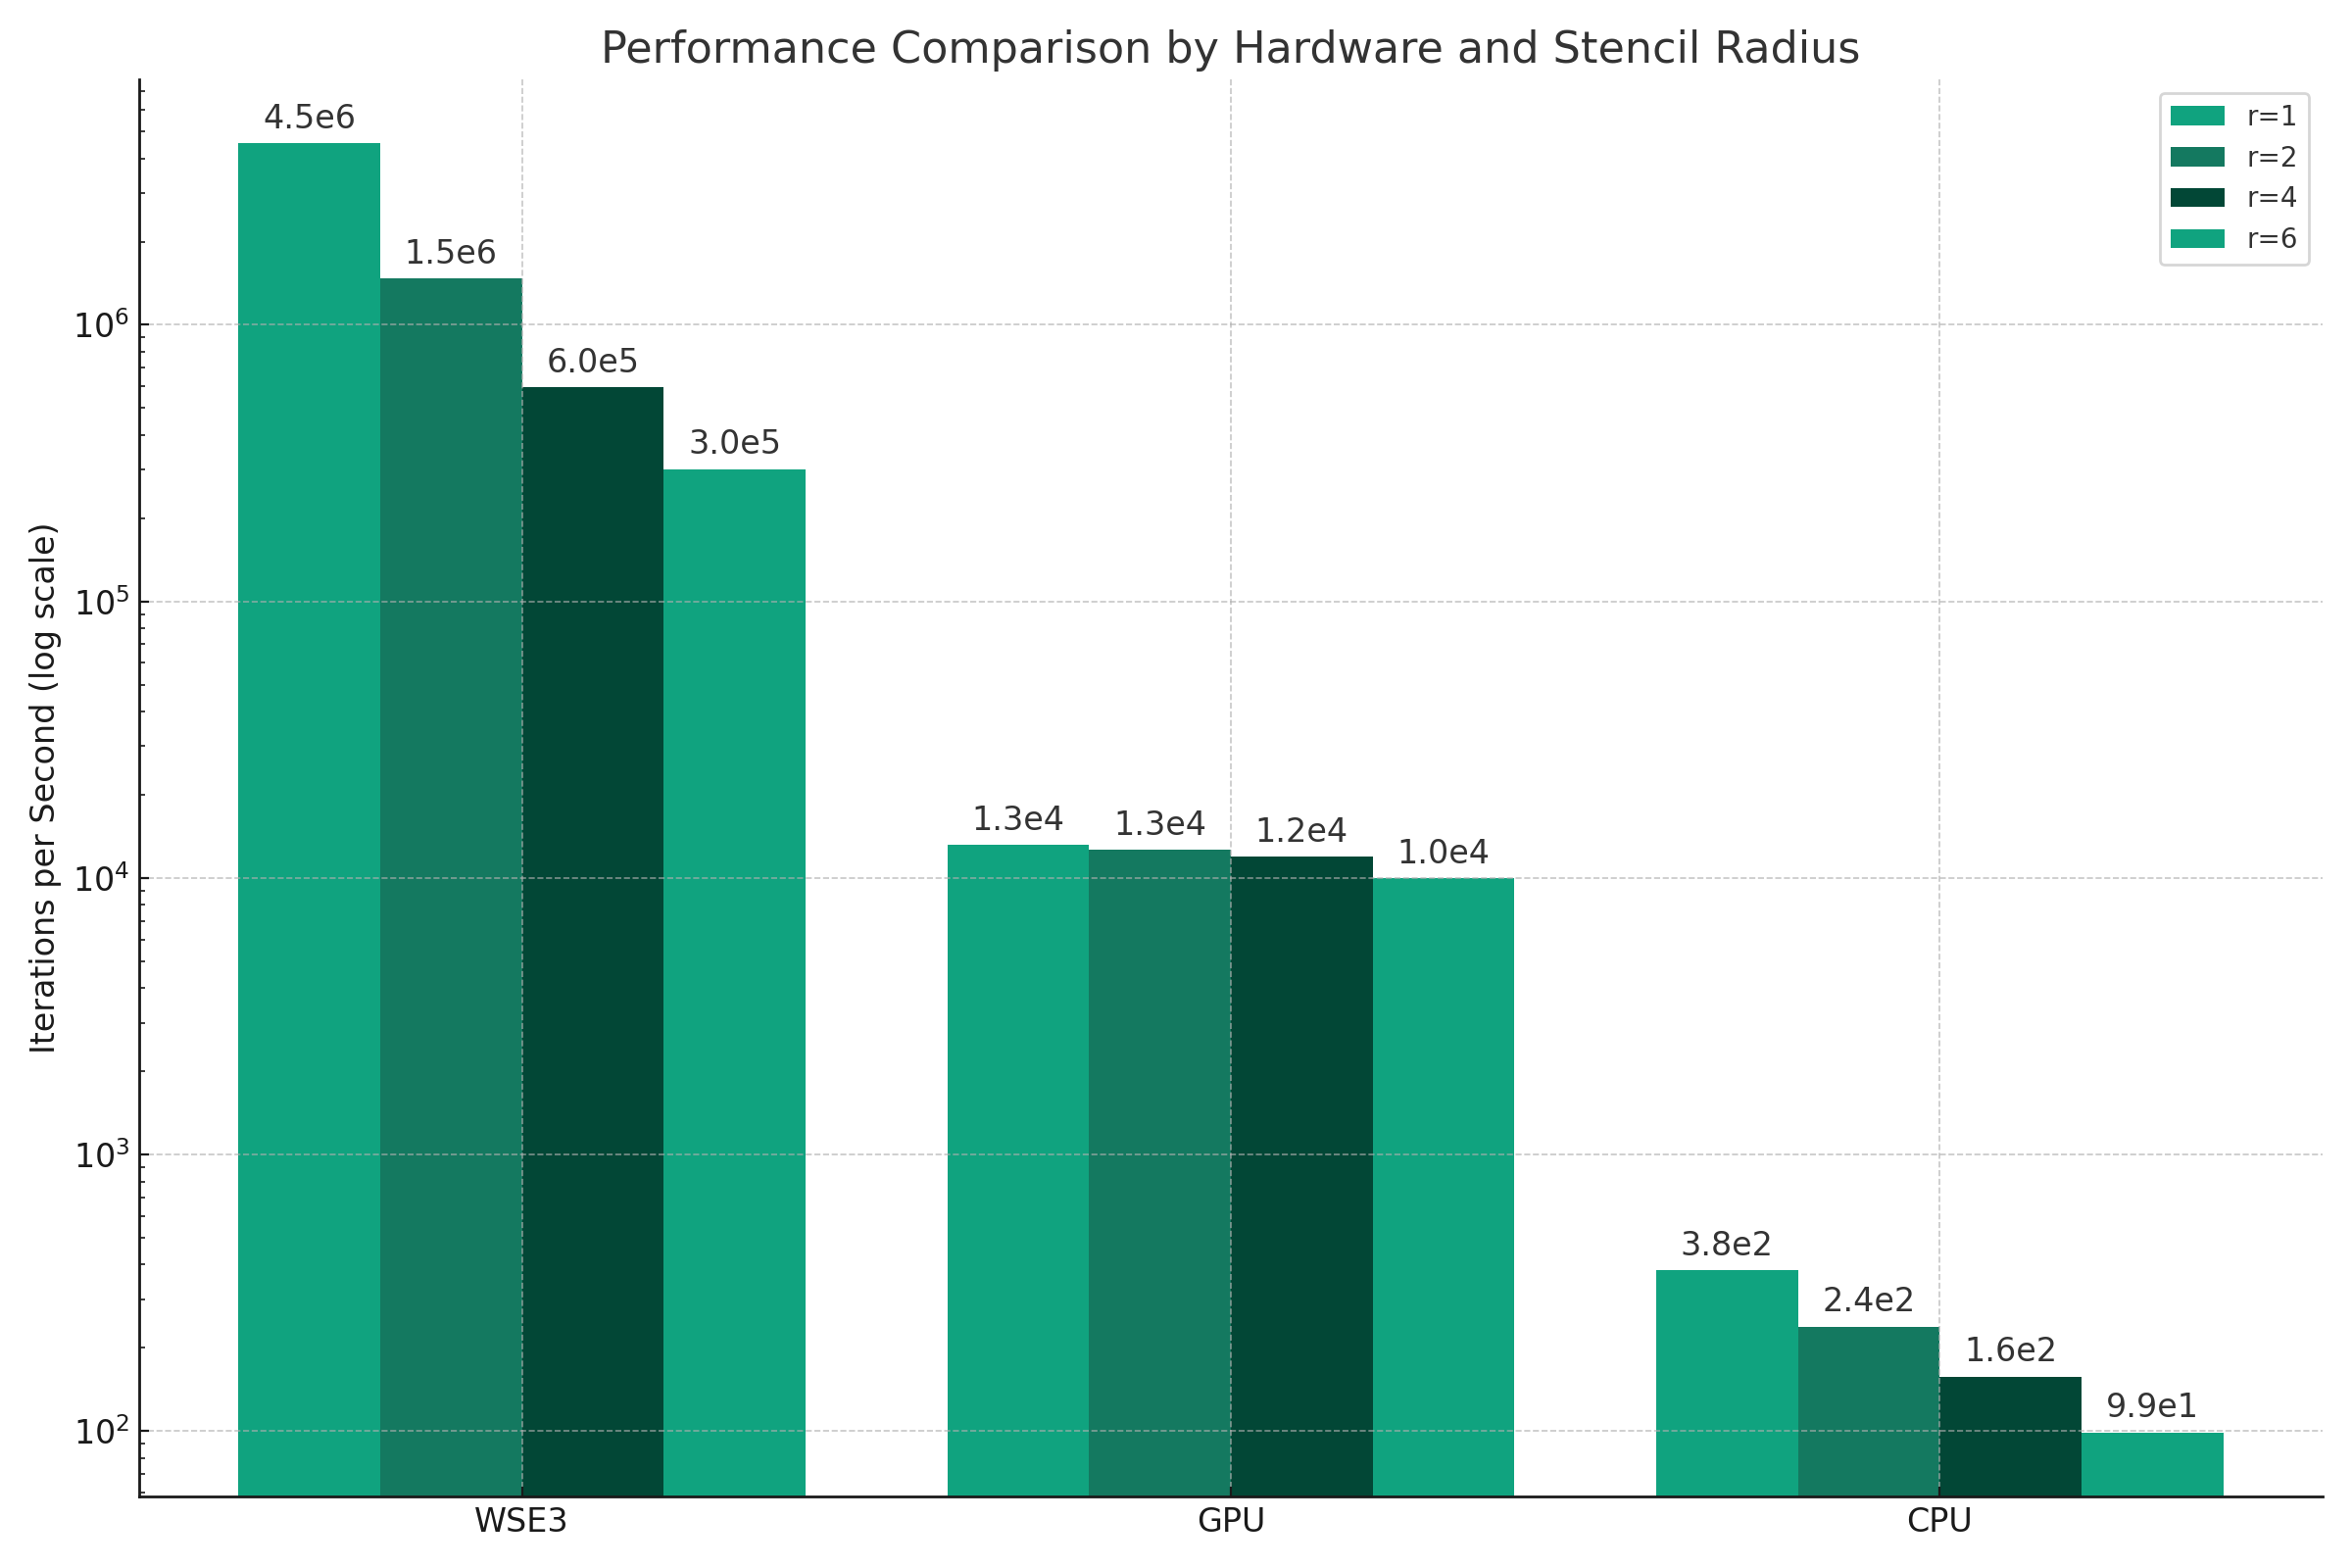
\includegraphics[width=0.5\linewidth]{cpu_gpu_cerebras_comparison.png}
    \caption{Performance comparison across architectures for a $10^3 \times 10^4$ grid. The Cerebras WSE-3 implementation significantly outperforms the \ac{gpu} (NVIDIA H100) and \ac{cpu} (AMD EPYC 9554) across all radii. While the \ac{gpu} performance is largely insensitive to the stencil radius, indicating a memory-bound workload, the \ac{cpu} and WSE-3 performance degrades as the computational cost increases.}
    \label{fig:cpu_gpu_cerebras_comparison}
\end{figure}

While the times for the \ac{gpu} and \ac{cpu} for this experiment where directly measured, we used the cycle count per iteration from the simulator for a significantly smaller grid size and a small iteration count, assumed perfect scaling to the full \ac{wse} dimensions as suggested from \autoref{sec:pe_overhead}, a constant cycle count per iteration and the clock speed of the \ac{wse} to calculate the time per iteration.

The speedup for radius 1 from \ac{cpu} to \ac{gpu} is about 40x. From \ac{gpu} to \ac{wse}-3 we observe an even larger speedup of about 358x. As the problem is compute bound on cerebras while it is memory bound on \ac{gpu}, the speedup for radius 4 from \ac{gpu} to \ac{wse}-3 is significantly smaller at about 53x

To evaluate the performance advantage of the specialized non-tiled algorithm, we compare it directly with highly optimized implementations on traditional \ac{hpc} architectures using grid sizes that match the \ac{wse} dimensions. This comparison uses the actual \ac{wse} grid dimensions as the problem size, which represents the maximum grid size achievable with the non-tiled algorithm.

For \ac{wse}-2 with dimensions $750 \times 994$ and \ac{wse}-3 with dimensions $750 \times 1200$, we measured the performance of the same radius-1 stencil on all three architectures.

\begin{figure}[h]
    \centering
    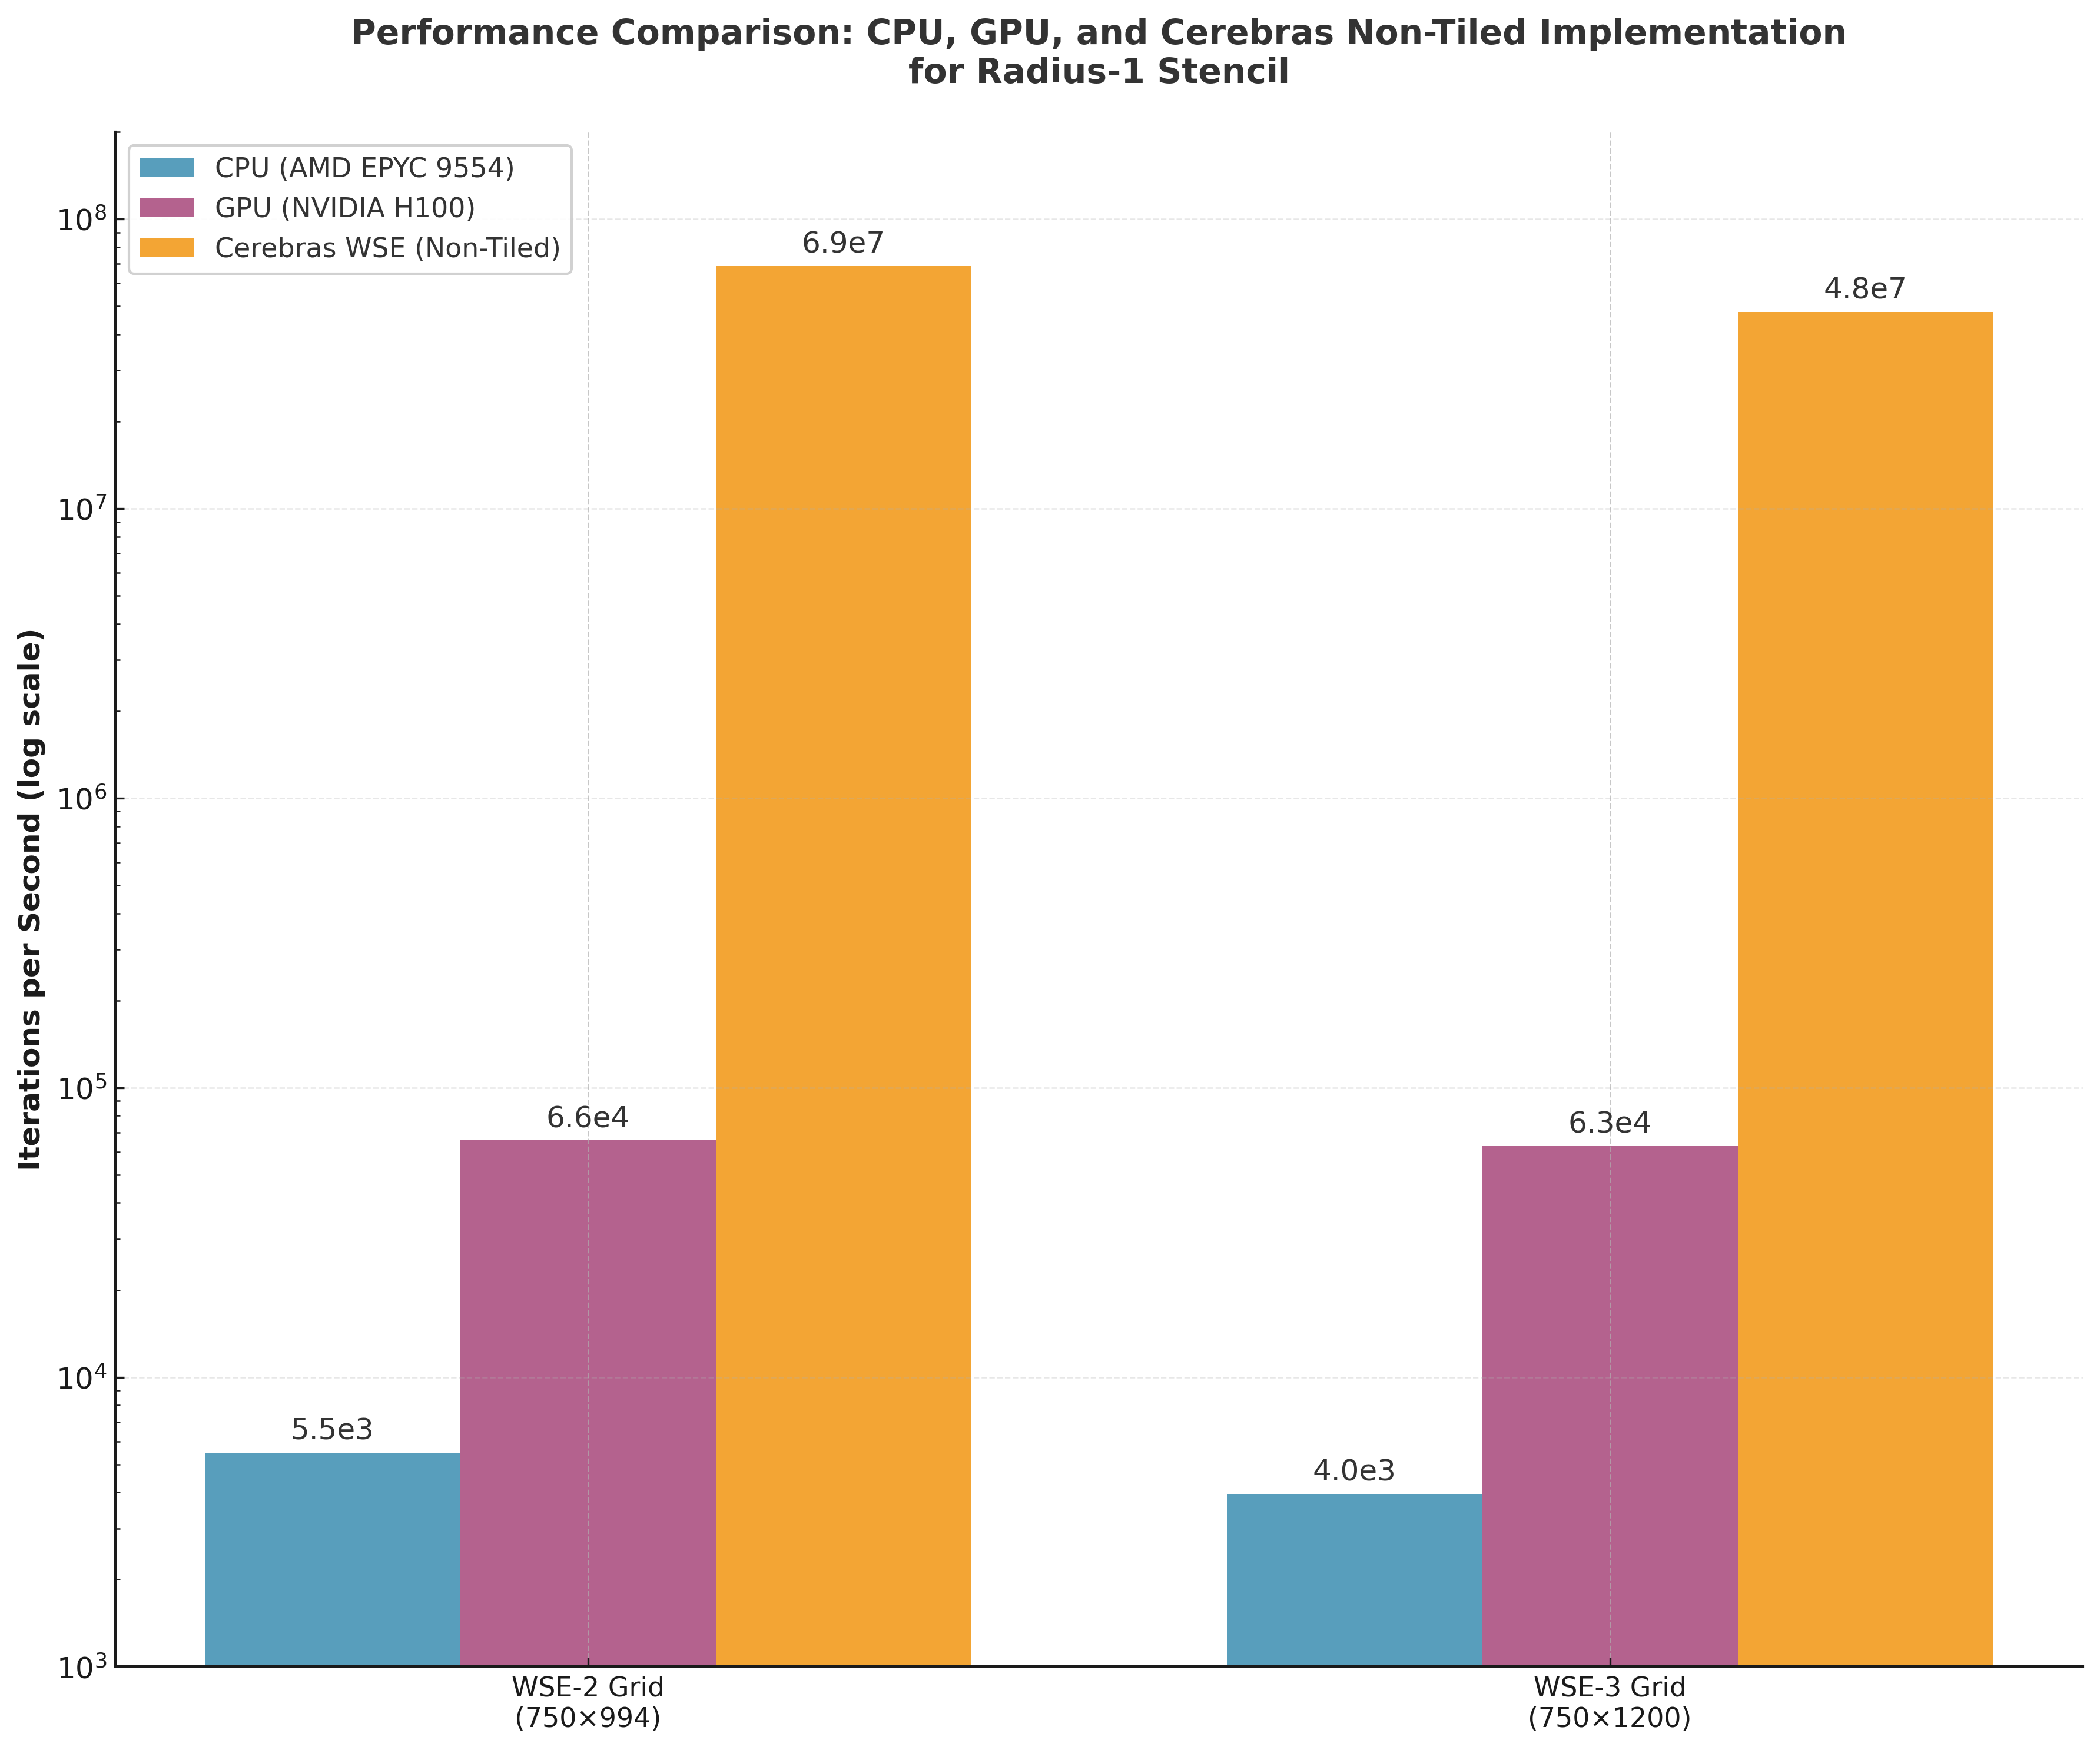
\includegraphics[width=0.7\linewidth]{cpu_gpu_cerebras_non_tiled_comparison.png}
    \caption{Performance comparison of the non-tiled Cerebras implementation against traditional \ac{hpc} architectures for radius-1 stencils. Results show iterations per second for grid sizes matching the \ac{wse} dimensions. The non-tiled algorithm achieves speedups of over 1000x compared to \ac{gpu} and over 12,000x compared to \ac{cpu}.}
    \label{fig:cpu_gpu_cerebras_non_tiled_comparison}
\end{figure}

The results demonstrate the exceptional performance of the non-tiled algorithm. For the \ac{wse}-2 grid size ($750 \times 994$), the Cerebras implementation achieves \num{68750000} iterations per second, compared to \num{65707} for the \ac{gpu}. This represents a speedup of 1046x.
For the \ac{wse}-3 grid size ($750 \times 1200$), the Cerebras implementation achieves \num{47826087} iterations per second, compared to \num{62743} for the \ac{gpu} with a speedup of 762x.

The performance advantage stems from the direct mapping of grid elements to \acp{pe}, enabling defacto in-memory computation with a memory that is significantly faster than the \ac{gpu} memory. While this approach is limited to grid sizes not exceeding the \ac{wse} dimensions, it provides unparalleled performance for problems that fit within these constraints.

\section{What contributes to the cycle count?}
We analyze the the instruction traces the simulator can record for what contributes to the the measured cycle counts.
We find that the effective simd width for some instructions in our implementation is lower than the theoretical maximum.
For \texttt{@fadds} it is 1.25 on wse-2 and 1.5 on wse-3.
The \texttt{@fmuls} instruction only have a simd width of 1 and we find that we measure exactly one cycle per instruction.

Here is a table that lists the different number of cycles per program segment. 